\documentclass[12pt,letterpaper]{article}
\usepackage[utf8]{inputenc}
\usepackage{mathptmx}
\usepackage{geometry}
\usepackage{fancyhdr}
\usepackage{hyperref}
\usepackage{graphicx}
\graphicspath{{./}}
\usepackage{listings}
\usepackage{subcaption}
\usepackage{lscape}
\usepackage{placeins}
\usepackage{titlesec}
\usepackage{float}
\titlespacing*{\section}{0pt}{1\baselineskip}{0.5\baselineskip}
\titlespacing*{\subsection}{0pt}{0.5\baselineskip}{0.5\baselineskip}
\usepackage{xcolor}
\hypersetup{
    colorlinks,
    linkcolor={red!50!black},
    citecolor={blue!50!black},
    urlcolor={blue!80!black}
}

%make url breaks
\def\UrlBreaks{\do-}

\newenvironment{myitemize}
{ \begin{itemize}
    \setlength{\itemsep}{0pt}
    \setlength{\parskip}{0pt}
    \setlength{\parsep}{0pt}
    \setlength{\topsep}{0pt}     }
{ \end{itemize}                  } 

\lstset{
	basicstyle=\small\ttfamily,
	showstringspaces=False}
\geometry{margin=1in}
\setlength{\emergencystretch}{3em}
\author{John Grando}
\title{CUNY MSDS Proposal}

\fancyhf{} % only used for clearing the headers
\rfoot{\thepage}
\pagestyle{fancy}
% --------------------------------------------------------------------
% Definitions (do not change this)
% --------------------------------------------------------------------
\newcommand{\HRule}[1]{\rule{\linewidth}{#1}} 	% Horizontal rule

\makeatletter							% Title
\def\printtitle{%						
    {\centering \@title\par}}
\makeatother									

\makeatletter							% Author
\def\printauthor{%					
    {\centering \Large \@author}}				
\makeatother							

% --------------------------------------------------------------------
% Metadata (Change this)
% --------------------------------------------------------------------
\title{	\Large { CUNY MSDS Capstone Project Summary} 	% Subtitle
		 	\\[2.0cm]								% 2cm spacing
			\HRule{2pt} \\						% Upper rule
			\LARGE \textbf{\uppercase{Commercial Building Energy Consumption}} \\ [0.25in] \Large \textbf{\uppercase{Analysis and Prediction}}	% Title
			\HRule{2pt} \\ [0.5cm]		% Lower rule + 0.5cm spacing
			\Large \today			% Todays date
		}

 \author{
		John Grando\\	
        john.grando@spsmail.cuny.edu \\
}


\begin{document}
%----------------------------------------------------------------
% Maketitle
%---------------------------------------------------------------
\thispagestyle{empty}		% Remove page numbering on this page
\printtitle					% Print the title data as defined above
  	\vfill
\printauthor				% Print the author data as defined above
\newpage
\pagestyle{fancy}
\setcounter{page}{1}		% Set page numbering to begin on this page
%----------------------------------------------------------------
% Begin document
%------------------------------------------------------------------------
\section*{Abstract}
Commercial Building Energy Consumption accounts for approximately 25\% of the United States energy production profile. Many economical and sociological factors are pushing owners of these buildings to reduce energy consumption and optimize performance. However, it is difficult to say whether a building is operating efficiently or not. Using publicly available data, models can be constructed to predict major fuel consumption. Keywords: building energy consumption, predicted energy consumption, baseline energy model.
\section*{Introduction}
Every few years, the U.S. Energy Information Administration (EIA) conducts a survey attempting to record pertinent features of these buildings, known officially as the Commercial Buildings Energy Consumption Survey (CBECS). While the survey is expansive (i.e. more than 600 tracked features), it is useful to identify predictors that significantly affect consumption. This study will focus on
creating a series of models to extract the most important survey questions and then use these values as predictors to train a final model that predicts fuel use consumption for standard practice buildings.
\section*{Data and Methods}
Due to the large number of features in the survey responses, it is not possible to analyze each one individually. Therefore, the first steps in the process will be centered around selecting smaller subsets from various feature extraction algorithms. The magnitude and contribution percentage of each variable will be considered in selecting features from this model. In order to try and
normalize the data, the response variable was divided by the gross floor area of the building and reported in in units of BTU per square foot (e.g. ELBTU/PerSF, NGBTU/PerSF). A neural network model will be built to take the subset of extracted features and make predictions for the selected major fuel use. A variety of hyperparameters will be tested, using cross‐validation, and compared on a common error metric. This step will reveal the optimal hyperparameter combination to use for the model.
\section*{Electricity Feature Extraction Results}
In order to rank the most impactful features, the variable importance metrics from the feature extraction models were all set to the same scale then summed and re‐normalized. It seems the attempts to create stratified random samples may have been beneficial in this case since there are some building type specific end‐uses that are highly ranked. For this fuel source, there are many attributes associated with refrigeration, office, and food sales equipment. Also, the attribute identifying one of the more atypical building types, speaking in an energy intensity sense, has made it
into the top 20 (PBA.5 [NON‐REFRIGERATED WAREHOUSE]). Additionally, some occupancy features (NWKERPerSf, FDSEATPerSf) have been included which is expected given that they impact interior space cooling and ventilation loads. In an attempt to truly follow the important predictors, no variables have been removed from this set and the order of importance remains unchanged.
\begin{figure}[h]
\centering
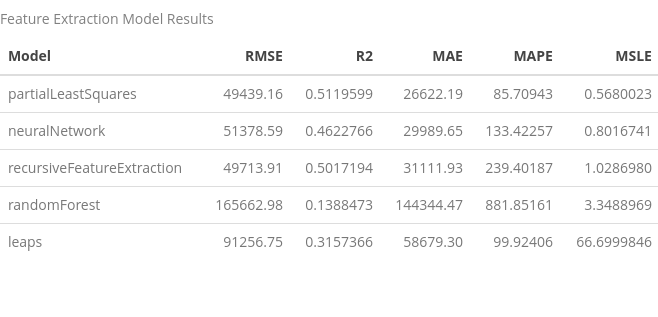
\includegraphics[width=.8\textwidth, height=0.25\textheight]{Images/electricity_psf_fe_summary.png}
\end{figure}
\begin{figure}[h]
\centering
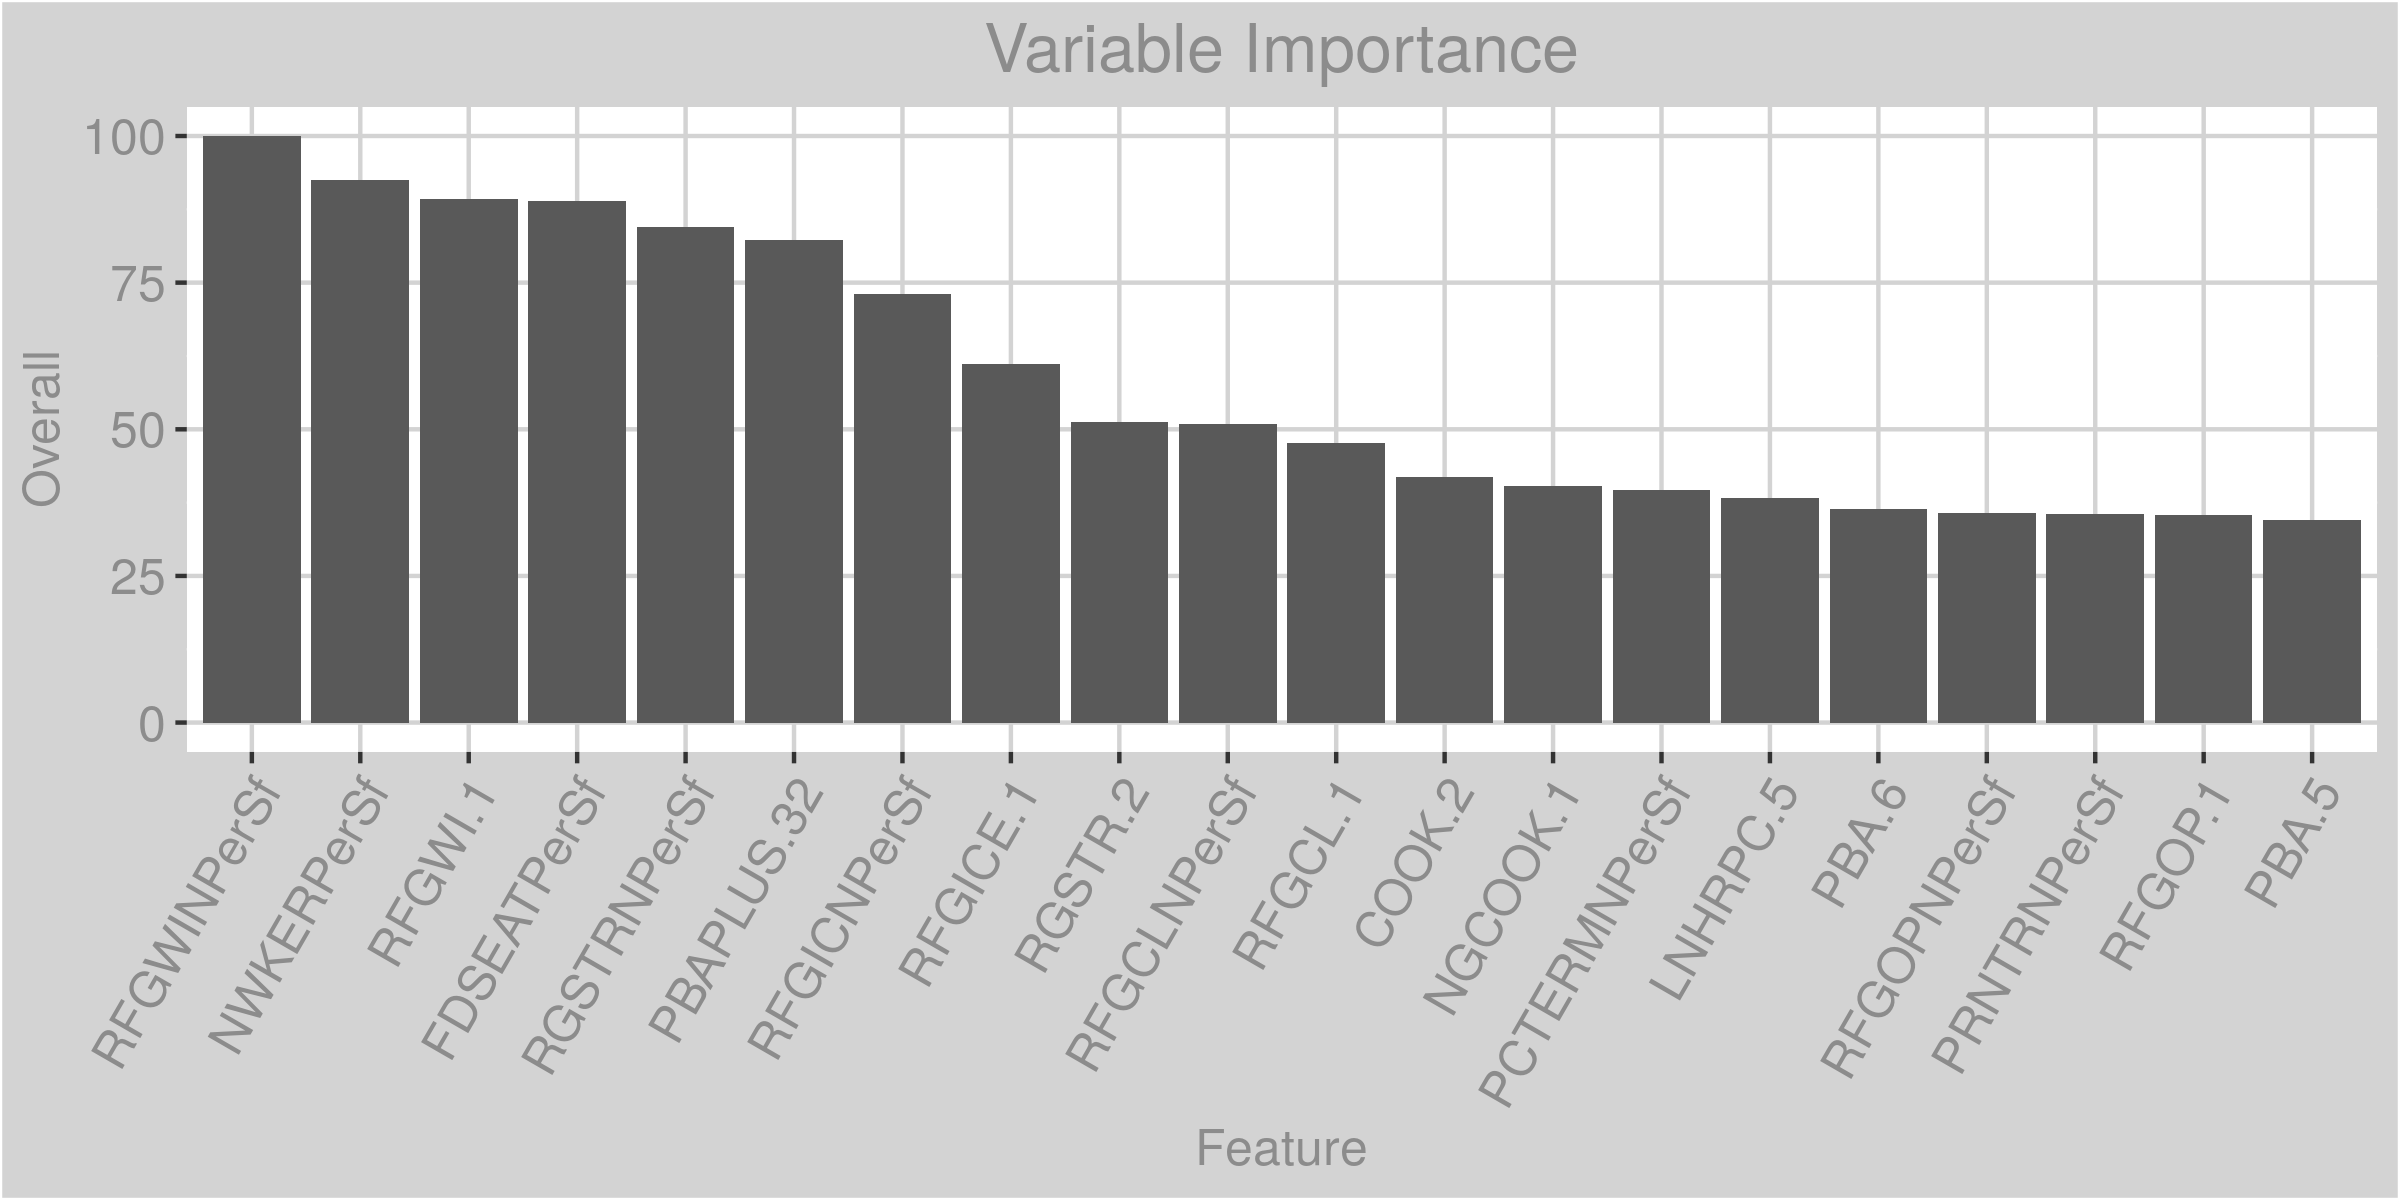
\includegraphics[width=.99\textwidth, height=0.375\textheight]{Images/electricity_psf_all_vars.png}
\end{figure}
\FloatBarrier
\section*{Natural Gas Feature Extraction Results}
As with the electricity results, attributes related to occupancy seem to have made a large impact, possibly due to the need to heat ventilation air, especially given some of these occupancy types are associated with 24/7 operation. Specifically, buildings which report a high density of food service seating appear to be directly correlated with high gas usage, which is not surprising. Also as expected, cooking and large heating equipment attributes are high on the list.
\begin{figure}[h]
\centering
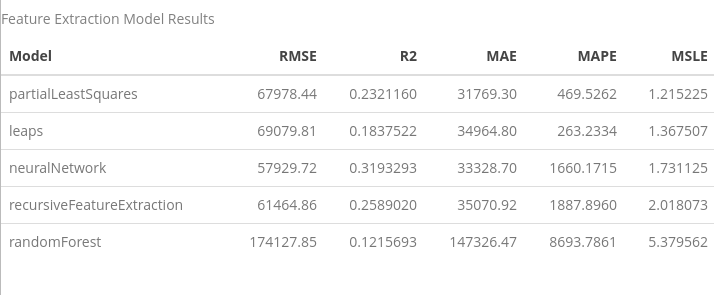
\includegraphics[width=.8\textwidth, height=0.25\textheight]{Images/natural_gas_psf_fe_summary.png}
\end{figure}
\begin{figure}[h]
\centering
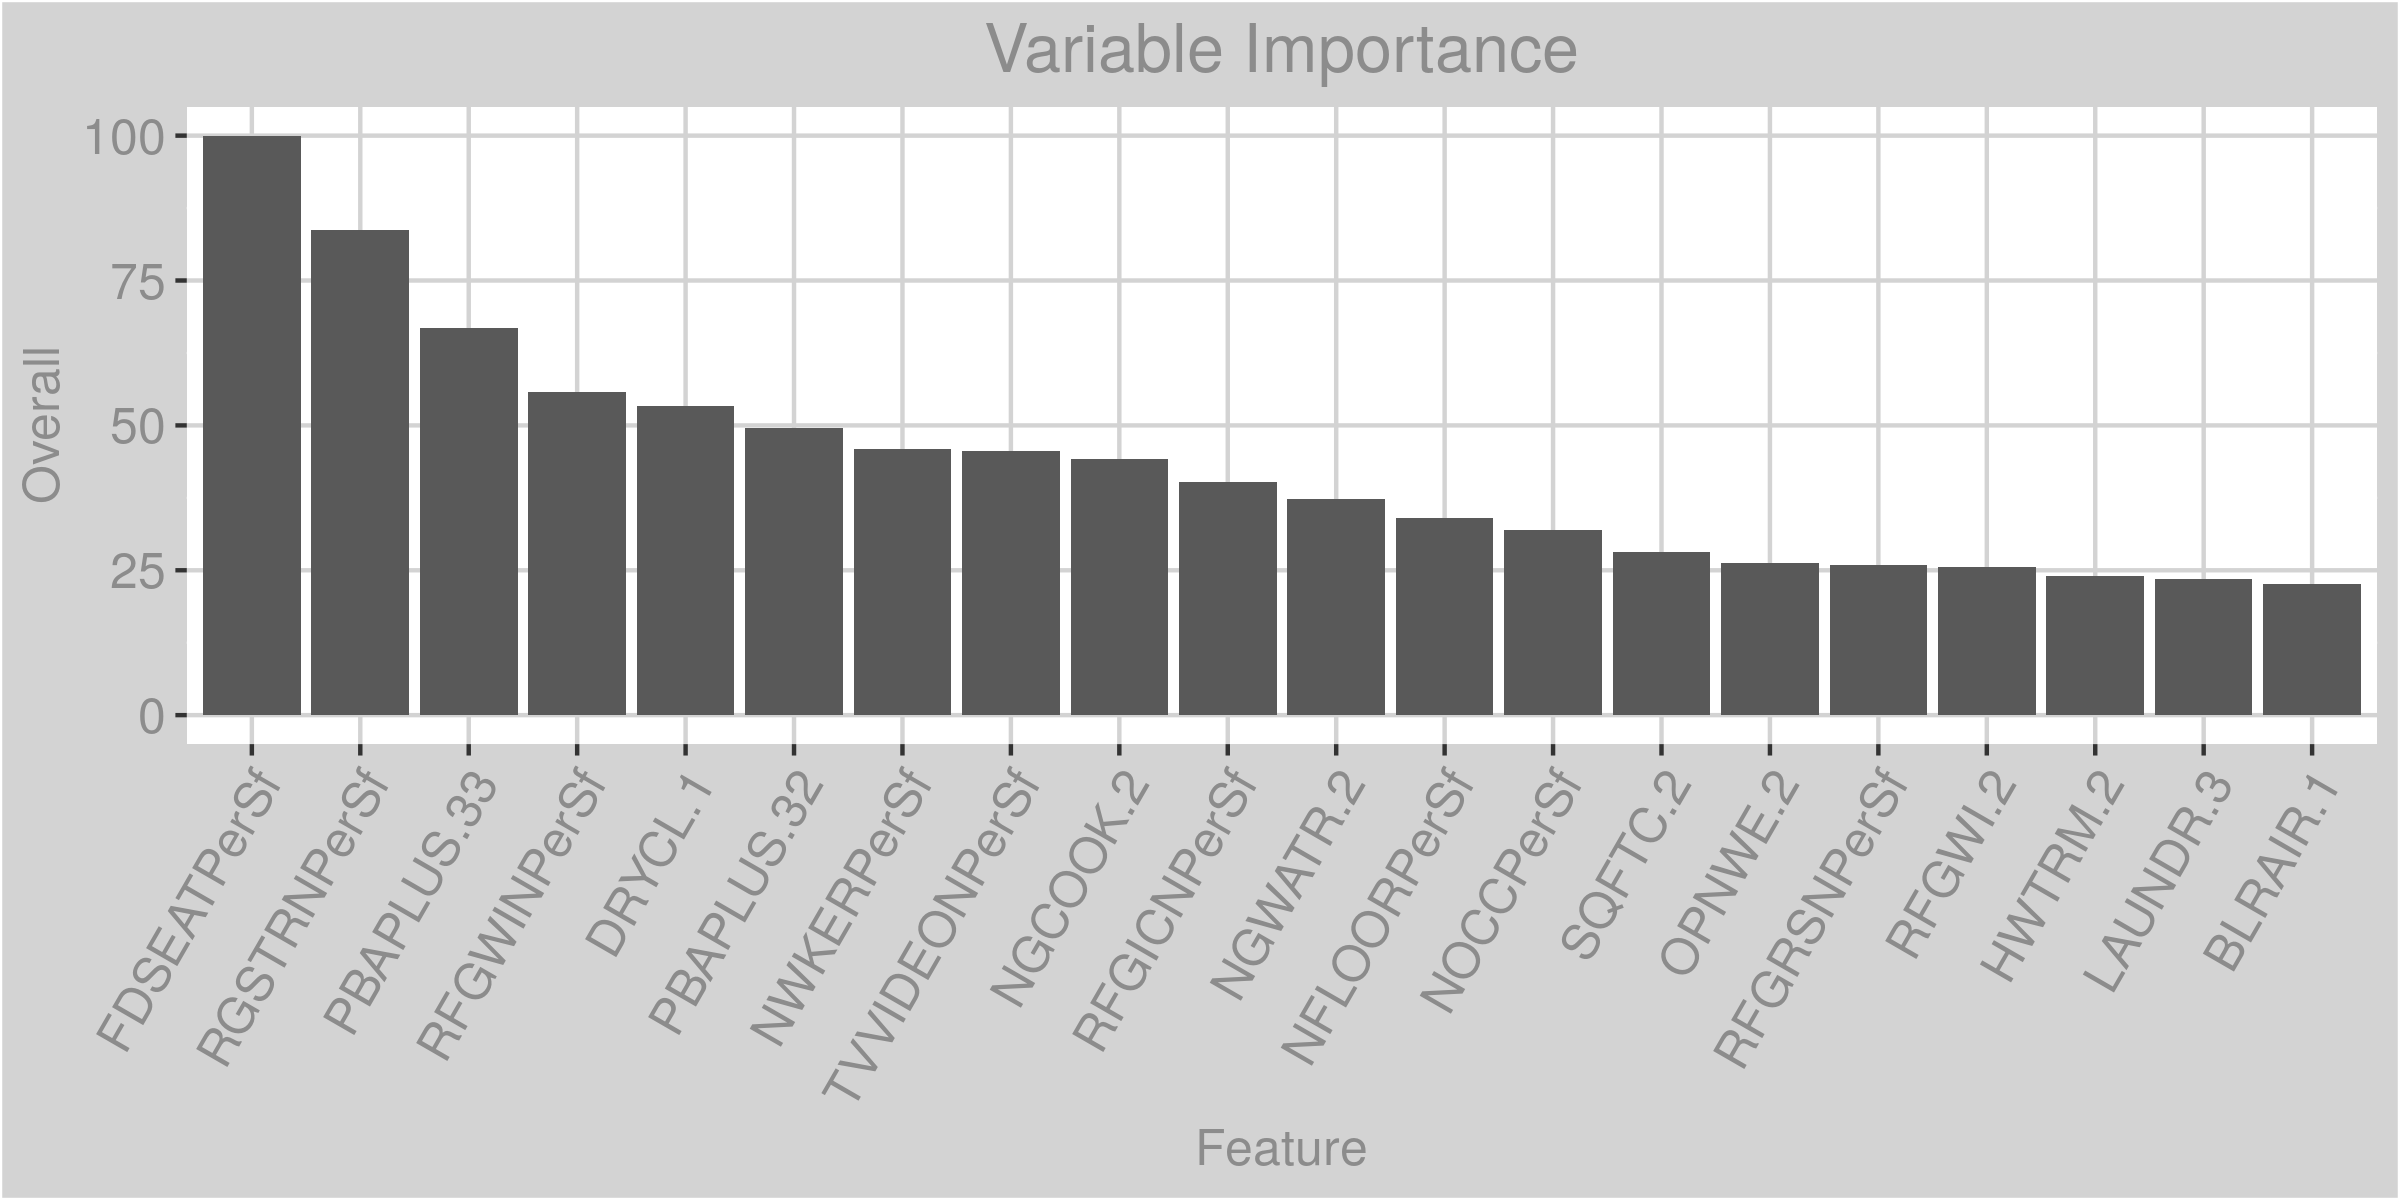
\includegraphics[width=.99\textwidth, height=0.375\textheight]{Images/natural_gas_psf_all_vars.png}
\end{figure}
\FloatBarrier
\section*{Neural Network Summary - Electricity}
The final selected model consisted of a 5 hidden layers, 1000 hidden layer nodes, a dropout rate of 0.3, no regularization, batch sizes of 150, using the rmsprop() algorithm with a learning rate of 0.0005, and 100 predictors. As can be seen in the graph below, the number of variables needed to obtain near‐peak performance, is much less than the full set.   The final selected
model, after re‐training, has a MSLE of 0.92 and RMSE of 54696. Comparing this model (’Full Neural Network’) to the previous feature extraction models, which used many more variables, the performance is competitive. Additionally, the results were then multiplied by their respect gross floor area and then compared to the set of feature extraction models, with the same transformation, in order to evaluate the total consumption prediction error. Again, it can be seen that this neural network model has shown to be competitive in this manner and, in fact,
has a better Rsquared value.

\begin{figure}[h]
\centering
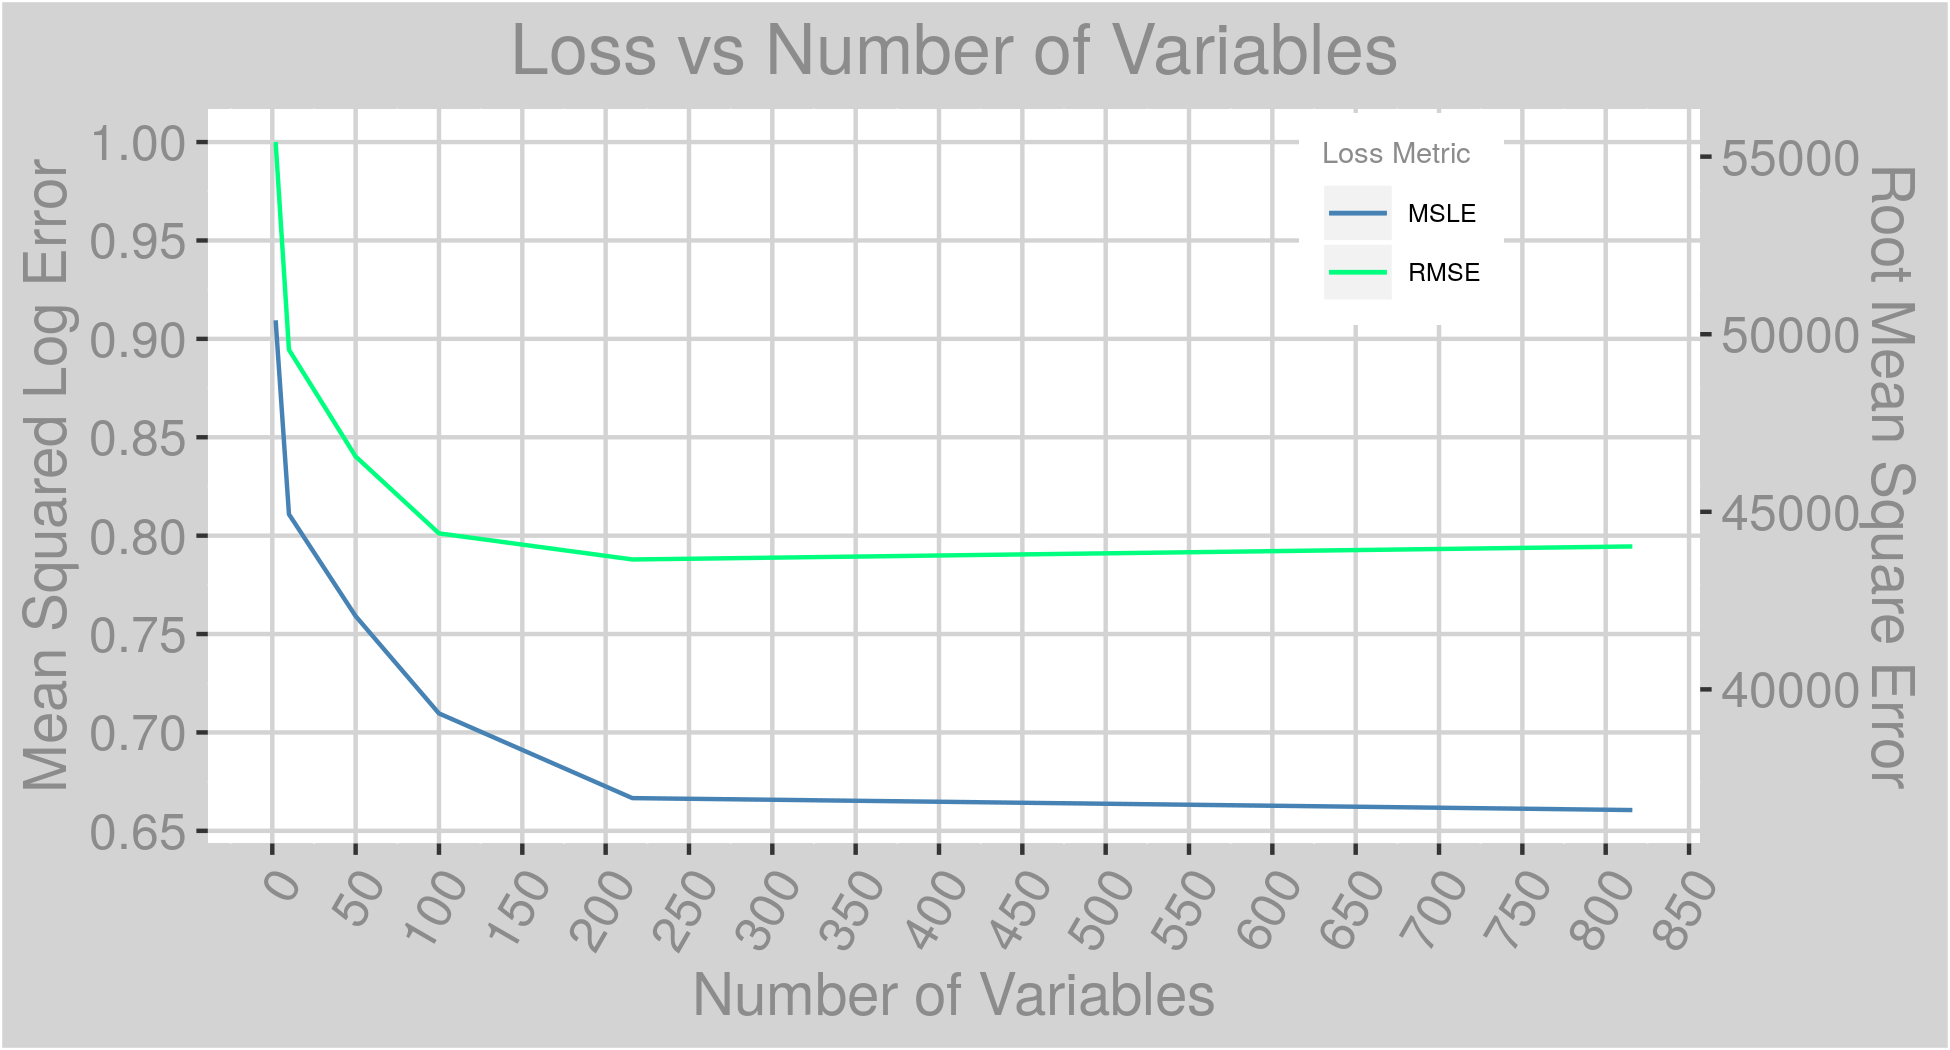
\includegraphics[width=\textwidth, height=0.3\textheight]{Images/electricity_psf_nn_error.png}
\end{figure}

\begin{figure}[h]
\centering
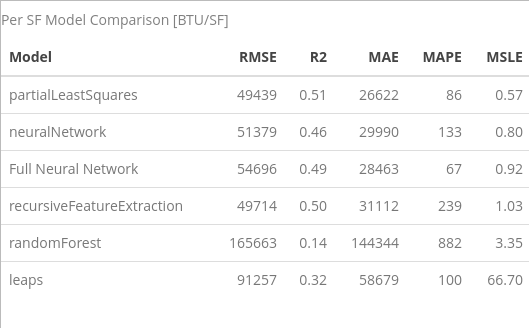
\includegraphics[width=.49\textwidth, height=0.3\textheight]{Images/electricity_psf_model_summary.png}
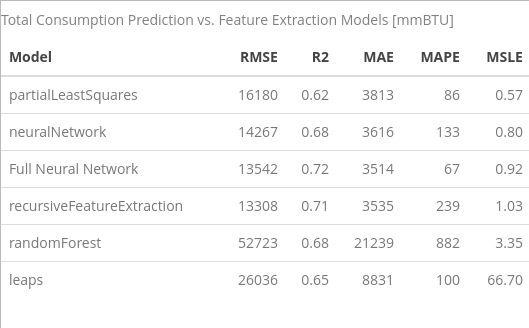
\includegraphics[width=0.49\textwidth, height=0.3\textheight]{Images/electricity_psf_model_summary_transformed.png}
\end{figure}

\begin{figure}
\begin{subfigure}{1\textwidth}
\centering
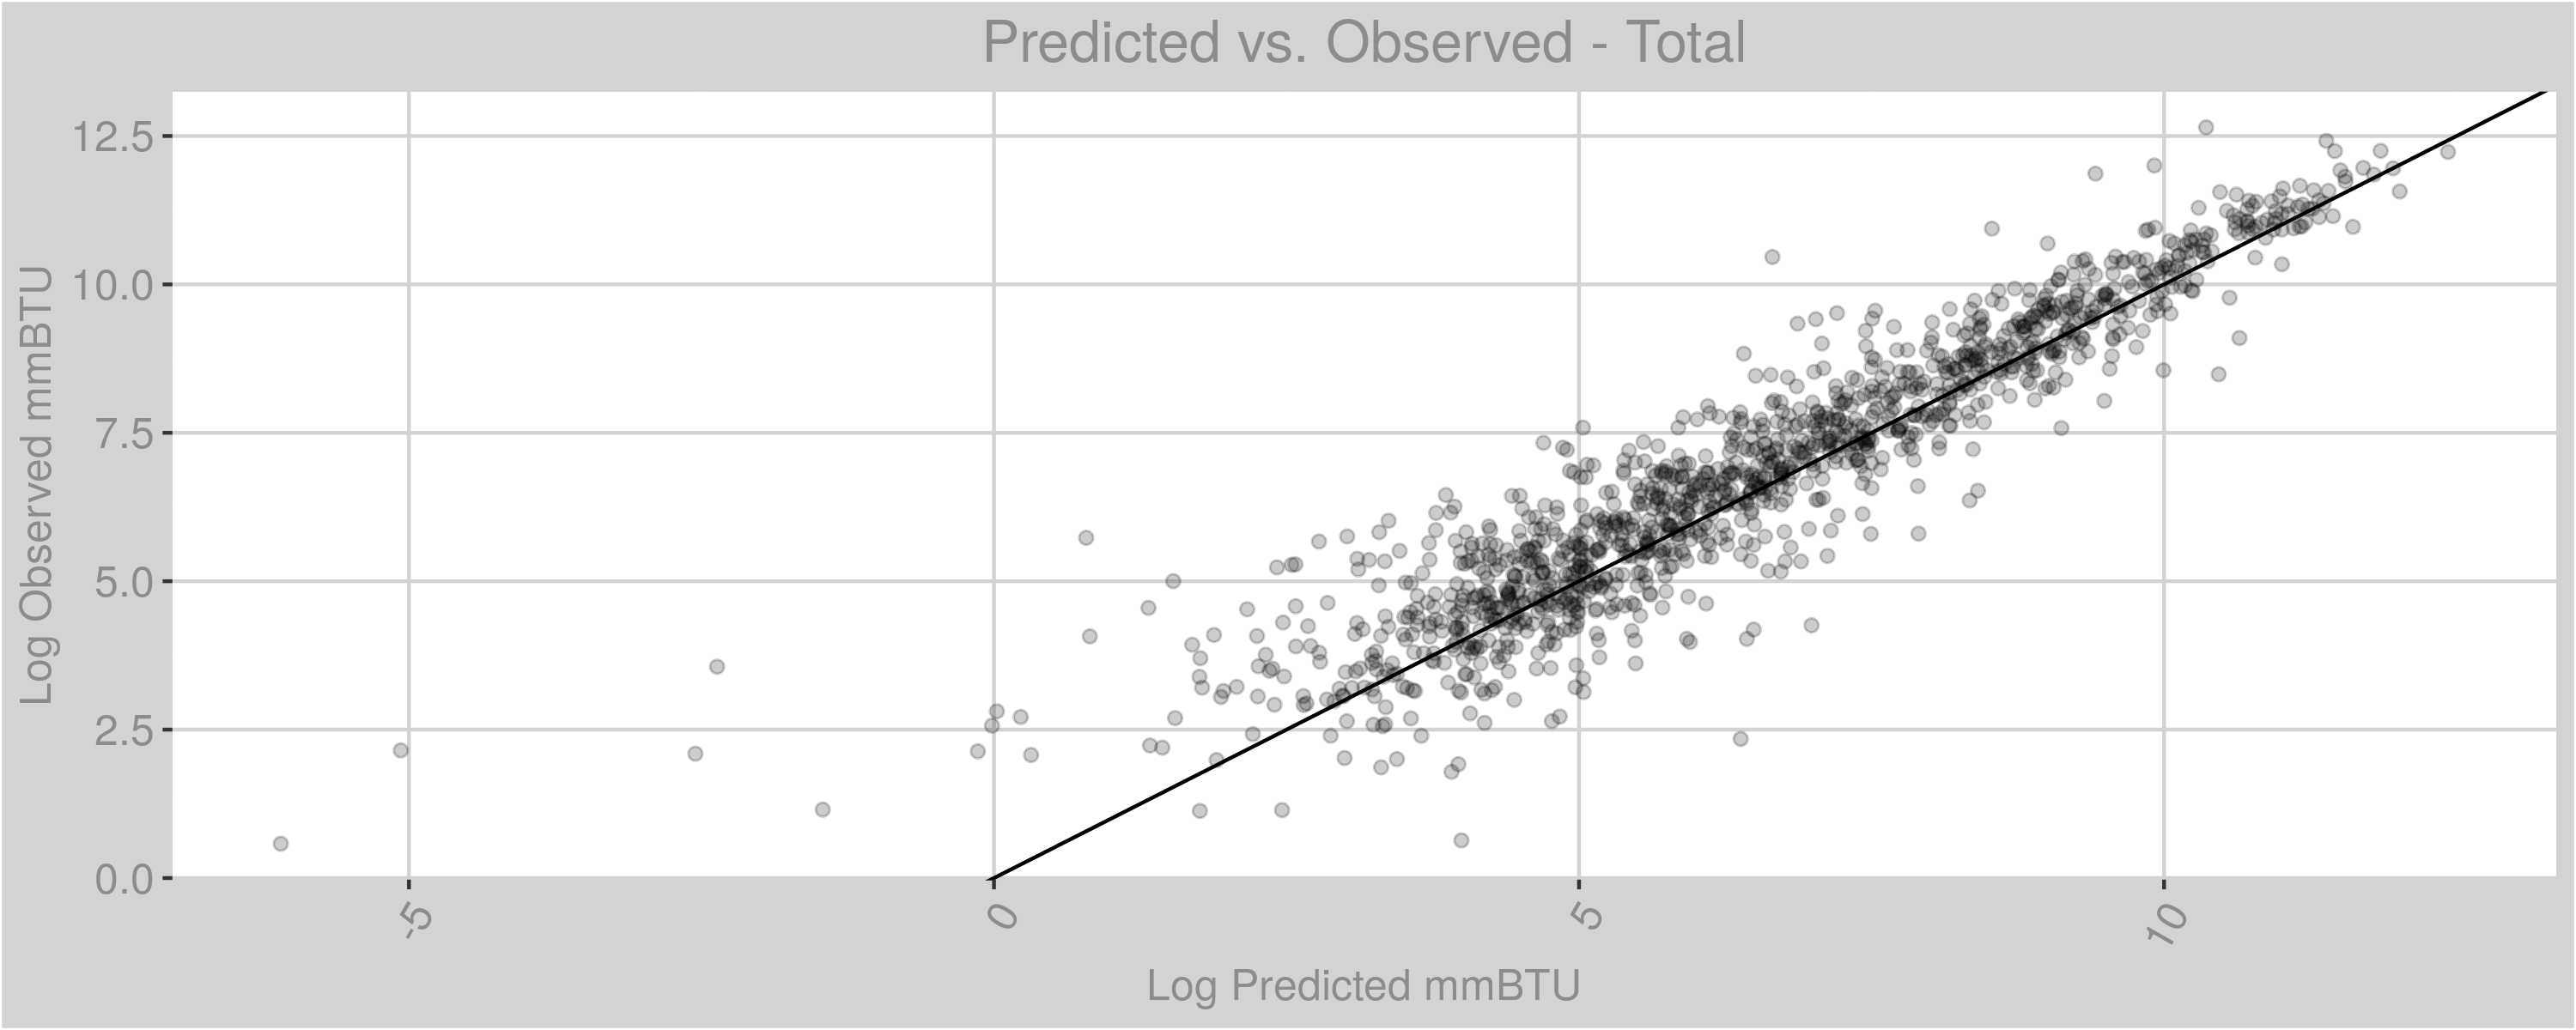
\includegraphics[width=.99\textwidth, height=0.3\textheight, origin=c]{Images/electricity_psf_nn_full_pvo_transformed.png}
\end{subfigure}
\end{figure}
\FloatBarrier

\section*{Neural Network Summary - Natural Gas}
The final selected model consisted of a 5 hidden layers, 800 hidden layer nodes, a dropout rate of 0.3, no regularization, batch sizes of 150, using the rmsprop() algorithm with a learning rate of 0.0005, and 100 predictors. As can be seen in the graph below, the number of variables needed to obtain near‐peak performance, is much less than the full set.   The final selected model, after re‐training, has a MSLE of 1.42 and RMSE of 61341. Comparing this model (’Full Neural Network’) to the previous feature extraction models, which used many more variables, the performance is actually better (when using RMSE).

\begin{figure}[h]
\centering
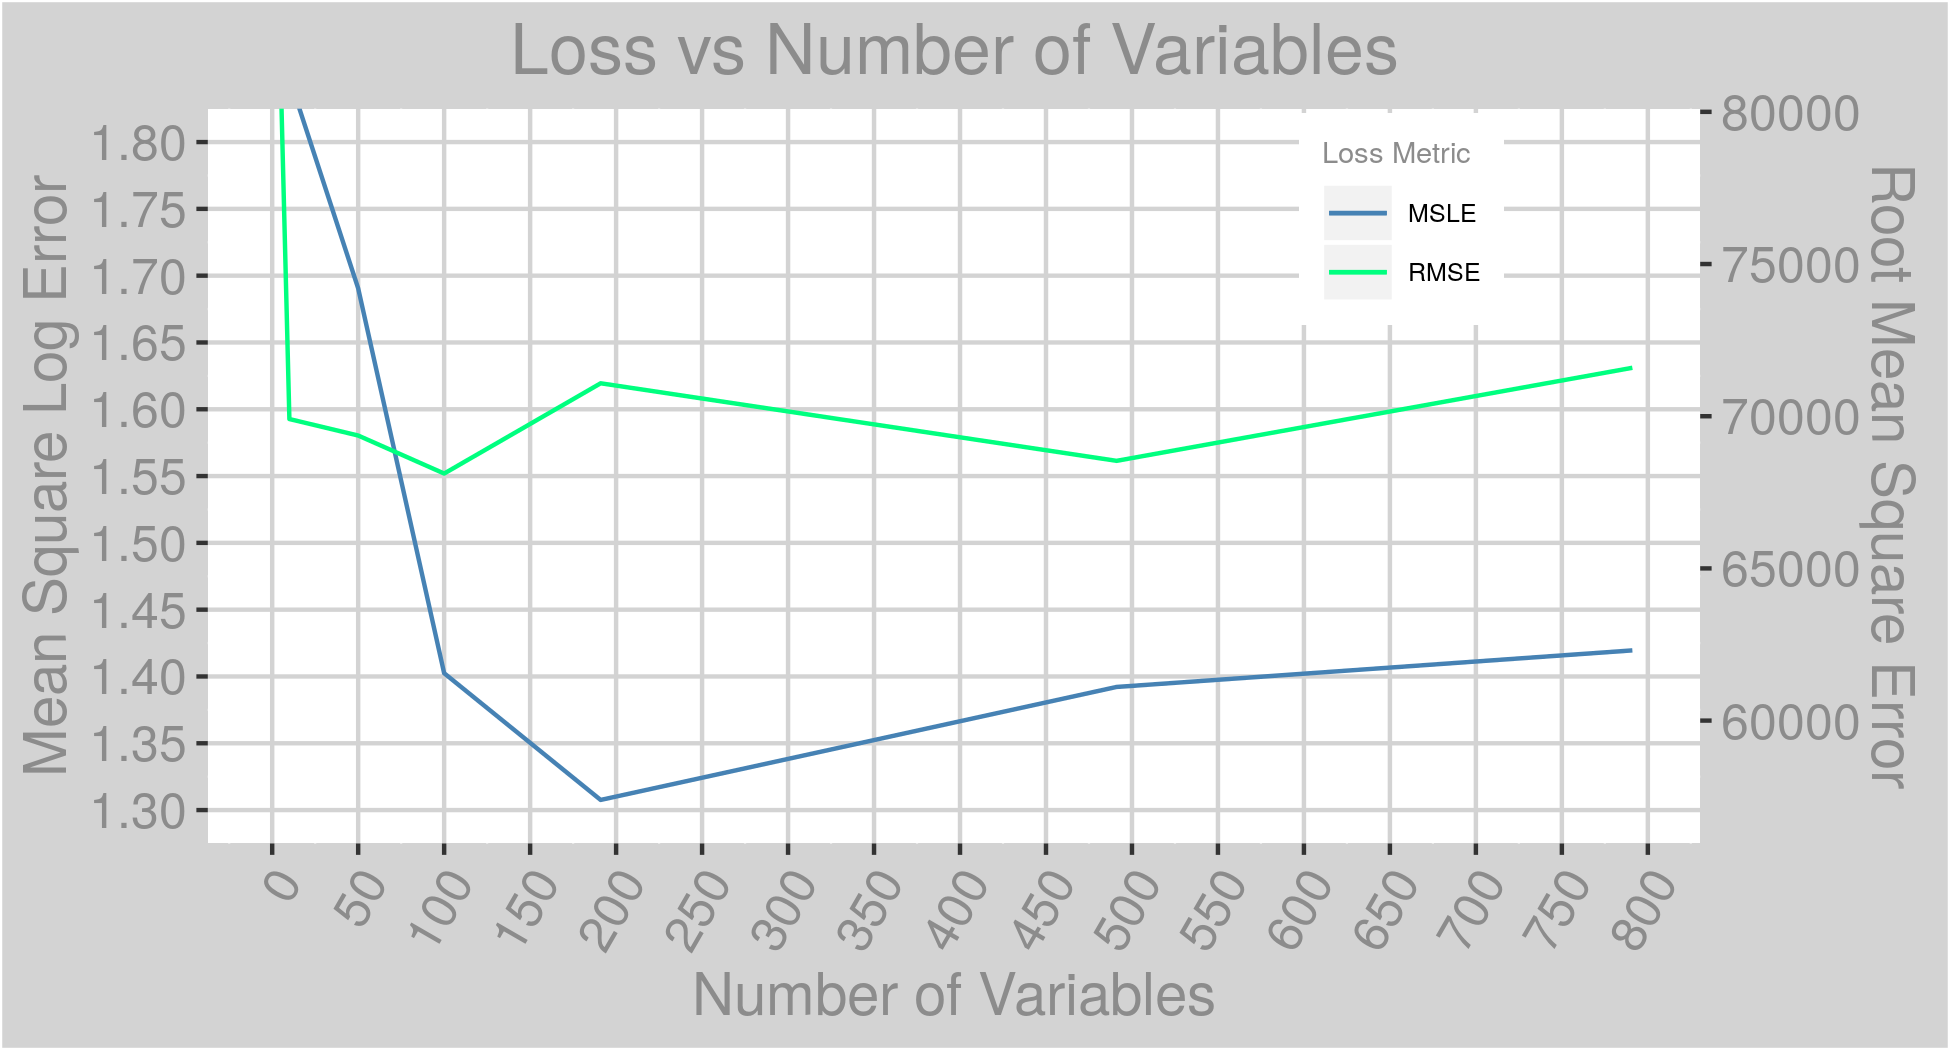
\includegraphics[width=\textwidth, height=0.3\textheight]{Images/natural_gas_psf_nn_error.png}
\end{figure}

\begin{figure}[h]
\centering
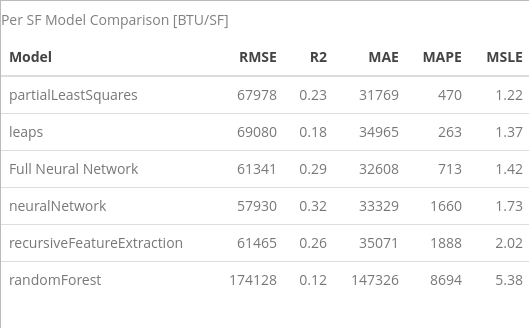
\includegraphics[width=.49\textwidth, height=0.3\textheight]{Images/natural_gas_psf_model_summary.png}
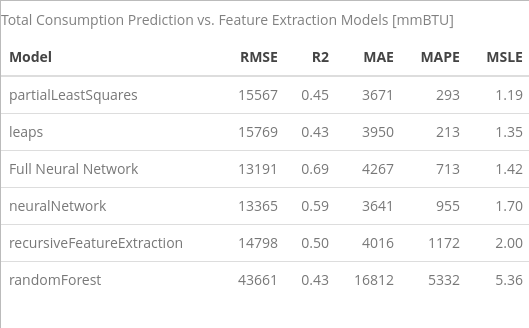
\includegraphics[width=0.49\textwidth, height=0.3\textheight]{Images/natural_gas_psf_model_summary_transformed.png}
\end{figure}

\begin{figure}[H]
\begin{subfigure}[H]{1\textwidth}
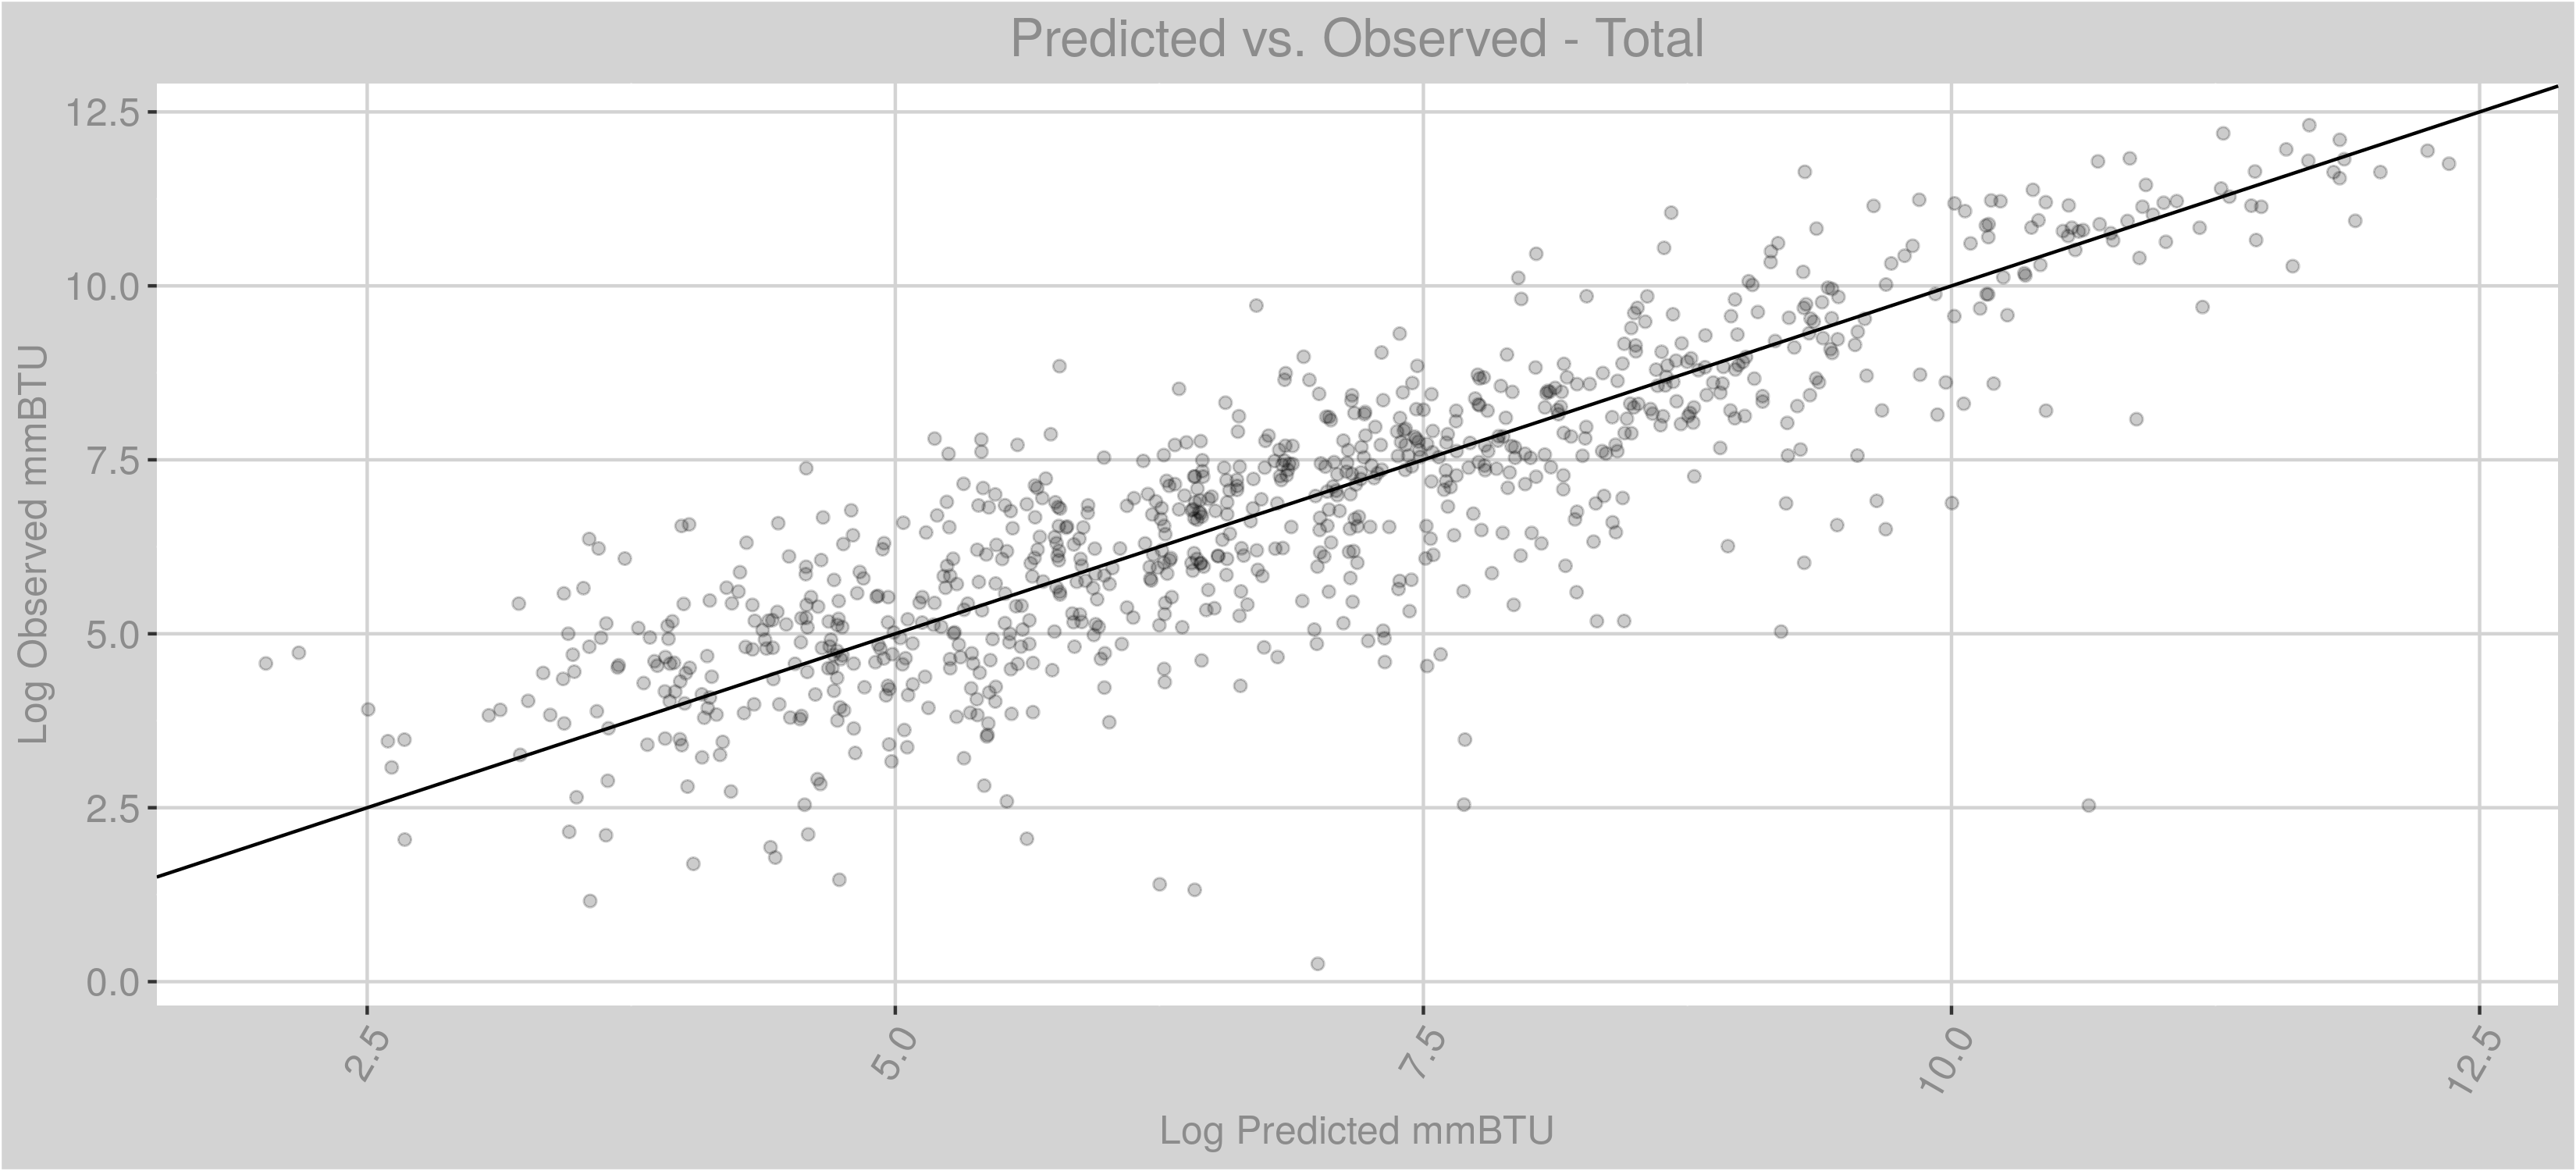
\includegraphics[width=.99\textwidth, height=0.3\textheight]{Images/natural_gas_psf_nn_full_pvo_transformed.png}
\end{subfigure}
\end{figure}
\FloatBarrier

\end{document}